\documentclass[11pt]{article}
\usepackage[utf8]{inputenc}
\usepackage{lipsum}
\usepackage[left=2cm, right=2cm, top=3cm, includefoot]{geometry}
\usepackage{comment}
\usepackage {graphicx}%Import images
\usepackage{float}%Set any float position of images for example.
\usepackage{titlepic}
\usepackage{multirow}
\usepackage{cite}
\usepackage {natbib}

\graphicspath{ {\Users\soren\Desktop\Projects 5. semester\Big Data/} }


%Allows for different colors in report
\usepackage{color}
\usepackage[dvipsnames, table, xcdraw]{xcolor}
\usepackage{tabu}
\usepackage{dcolumn}
\newcolumntype{A}{D{.}{.}{2.3}}
\setlength{\parindent}{0pt}


%Setup allows for clickable ToC with different colors
\usepackage{hyperref}
\hypersetup{
    colorlinks,
    citecolor=black,
    filecolor=black,
    linkcolor=black,
    urlcolor=black
}


% Header and Footer Stuff
\usepackage{fancyhdr}
\pagestyle{fancy} %Use fancy page style
\fancyhead[R]{CBS} %Align to the right on the page
\fancyfoot{}
\fancyfoot[R]{\thepage\ } %Align to the right on the page
\renewcommand{\headrulewidth}{0.5pt} %overwrite headers width
\renewcommand{\footrulewidth}{1pt}  %overwrite footers width




\begin{comment}
Renew command overwrites a previous function. Therefore, it is used to overwrite the header and footer width.
fancyfootHDR package, allows us to add cool headers and footers. R aligns to the right  \thepage\ references the actual page number.
\end{comment}




\begin{document}





%Start of titlepage
\begin{titlepage}
	\begin{center}
	\line(1,0){300} \\
	[0.25in]
	\color{NavyBlue} \huge{\bfseries A Big Data Research Paper } \\   
	[2mm]	
	\color{black}
	\line(1,0) {200} \\
	[0.1cm]
	\color{black}\textsc{\LARGE On Donald J. Trump's Twitter Activity} \\
	[0.75cm]
	\textsc{\LARGE Copenhagen Business School} \\
	[9.5cm]




\end{center}



\begin{figure}[H]
	\centering

%
 %\raisebox{20mm}[0pt][0pt]{
 %\makebox[\textwidth][c]{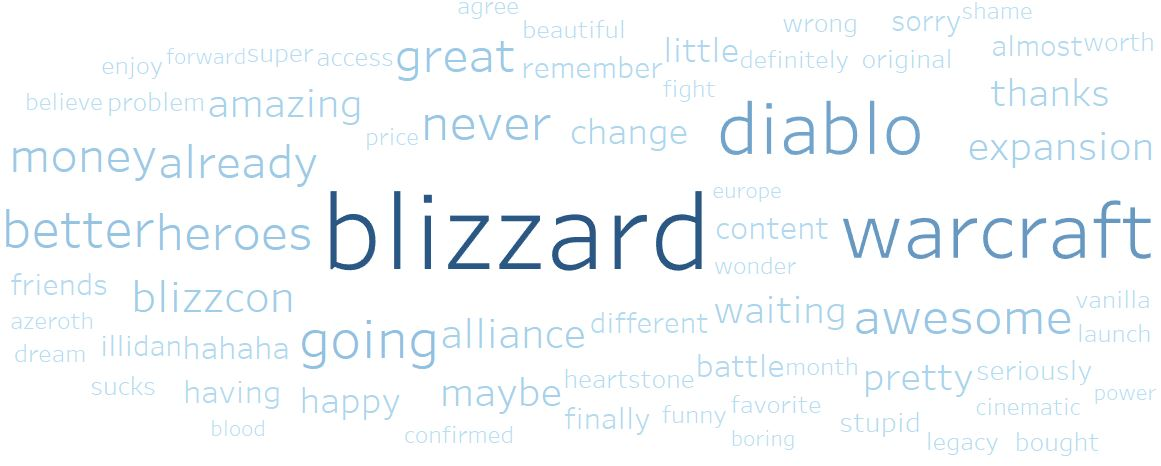
\includegraphics[scale=.55]{BlizzardWord2Cloud.PNG}
 %}}

\vspace*{-12cm} 
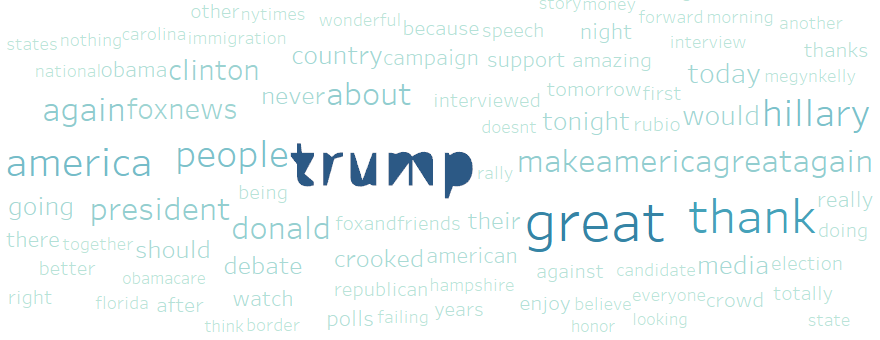
\includegraphics[scale=.75]{TrumpWord.PNG}



\caption{ Trump Wordcloud }
\vspace*{1.25cm} 


\end{figure}


	\begin{flushright}
\vspace*{1.25cm} 

	\textsc{\large Søren Kolbye Jensen \\}
	Bsc. Ha(IT) \\
	\#43124133123 \\
	December 1, 2017
	\end{flushright}





%End of titlepage
\end {titlepage}



%Table of contents & summary
\color{NavyBlue} \tableofcontents \color{black}
\thispagestyle{empty} %Remove the header, by removing all the style
 \cleardoublepage
\setcounter{page}{1}%Reset page counter at introduction page 
\pagenumbering{arabic}
%\addcontentsline{toc}{section}{\numberline{}Summary}


\cleardoublepage%Table of contents end


\section{Abstract} %Summary
The topic in this research paper is an analysis of Donald J.\ Trump's Twitter account, using datascience and datamining tools to reveal his behaviour.\
Problemformulation
The research questions that will be answered in this paper are:  \\

 What was trump's behaviour on social media, prior to his announcement of his presidency.\ And how did it change, during and after his political campaign.\ \\
 How does Trump's behaviour affect the stock prices of companies ?\\
 What does using datascience to analyze Donald Trump?s behaviour mean from an ethical standpoint?\\
 
 The research questions were answered using datasets from Trump's twitter profile, as well as nasdaq to get stock prices of companies he tweeted about.\
 

\cleardoublepage %Summary end


%End of table of contents & summary









%Start of report






%Start of introduction_____________________________________________


\color{NavyBlue} \section{Introduction} \label{sec:intro}

\color {black}

Big Data has changed how data is viewed in society, businesses have invested heavily in infrastructure that can improve data collection.\ This new infrastructure makes it possible to use big data to analyze the behaviour of individuals on social media channels, such as Twitter, Facebook and Instagram.\ \citep{foster}\ However, the vast amount of data available with modern technologies has proven difficult to analyze.\ According to Andrew McAfee and Erik Brynjolfsson, big data can be either structured or unstructured.\ The determining parameters are "Volume, Velocity, and Variety". \citep{velocity}\ In order to surmount  this difficulty,  the emerging field of data analytics is implementing what is called "Data Science" and "Datamining".\ \\

According to Foster Provost and Tom Fawcett , datascience and datamining are related, but not the same.\  Data science is the act of using fundamental principles, to guide extraction of knowledge from datasets and  Datamining deals with extracting knowledge from data using technologies, which incorporates the principles of data science.\ \citep{foster} \\

This research paper aims to use some of the fundamental principles of data science in conjunction with datamining technologies.\ This will be done in order to analyze the behavior of U.S president Donald J.\ Trump.\ and how this behaviour changed during his political campaign, as well as how his behaviour affected the U.S.\ financial markets.\ Therefore, the motivation behind this research, is to see how data can reveal a top politicians behaviour and thus also discover the actual benefits of data analysis. 


\subsection{Case introduction}
Donald John Trump, born in 1946 in Queens. New York, is the president of the united states and the CEO of the Trump Organization. On june 16th, 2015, Trump officially announced his candidacy as the 20th US President". This political campaign was heavily involved with social media, as Trump was actively fighting big news channels, such as CNN, BBC etc. labelling them as "fake news". Thus, Trump figured out a way to distribute highly controversial statements and gain political support by his use of social media channels such as Twitter. Trump himself describes social media as a "key role" in winning the presidency on November 9th, it is therefore important to investigate how data science can help analyze his behaviour and impact on such social media channels.


%http://www.bbc.com/news/entertainment-arts-37952249
%https://www.cbsnews.com/news/president-elect-trump-says-social-media-played-a-key-role-in-his-victory/

%End of introduction________________________________

%https://www.aol.com/2016-election/timeline/
%https://www.dropbox.com/sh/kd87npmrvcwiyge/AADRTmSB6lDt5ChunVY_Xy0Ea/ExampleProjects?dl=0&preview=ExampleProject%2301-VisualAnalytics-NYC_TaxiRides-GreenCabs_vs_Uber.pdf

\section{Problem Formulation and Research Questions} \label{sec:ch1}
From the case introduction a couple of research questions have been developed. Therefore, to summarize:  The goal of this research paper is to analyze  trumps behaviour on Twitter and how he used Twitter for political endeavors. A visual analysis on his behaviour between 2009 and 2017 will be conducted to reveal the patterns in his behaviour in this timeframe. This leads to the research question: 

\par\vspace{10pt}

What was trump's behaviour on social media, prior to his announcement of his presidency and how did it change after his announcement?.\\

In addition to this, due to Trump's political position, it would be interesting to investigate the impact that his tweets has on the stock-price of companies, during his campaign he has posted both good and bad things about numerous companies. It is therefore relevant to investigate, if his Tweets have an impact and if that impact is short-term or long-term. The company picked for this research question, is lockheed-martin. This leads to the research question:\\

How can a negative tweet from Donald Trump affect the stock prices of companies ? \\

Finally, it is relevant to evaluate and discuss what the above actually means to the context of Data Science, both from an ethical point of view, but also from a practical point of view. This leads to the final research question: \\

What does using datascience to analyze Donald Trump's, or any other individuals behaviour, mean from an ethical standpoint?
 
\subsection{Delimitations}
Due to this not being a statistics course, in addition to the fact that statistics is not being taught on ha(it.), I will not dwell too much into the deeper statistical details of my datamodels. Furthermore, concepts such as R-squared,  and other metrics are only barely mentioned in the course litterature. In spite of this, I will attempt to give light explanations of these metrics using other sources, because I believe it is one of the fundamental skills that a data scientist should posses.

\section{Conceptual Framework}
In this section I will discuss my conceptual framework which I used in order to investigate the research questions using data science.

\subsection{Supervised datamining}
Supervised and unsupervised datamining comes from machine learning, in a supervised method the data scientist will "supervise" the data and provide target information. In this research paper I have chosen to use supervised datamining, because there is a specific target (e.g. The predicted stock price of a company).  There are two "main" subclasses when it comes to using supervised data mining. One is classification and the other is regression - these two differ in terms of what the target is. In this research paper, the target is stock prices and thus it can be defined as a numeric target. The other main subclass of supervised datamining is classification which deals with binary targets, however this has not been used in the research paper. I will use supervised datamining methods, because my target is specified and the data on said target exists. Furthermore, the historical data of the stock value of the examined company is complete.


\subsection{Linear regression and fitting}
In this research paper, models containing linear regressions will be used, in order to discover the relationship among variables in the data model.  This will help create a simple predictive model of the datasets showcasing Trump's short-term impact on certain companies, when he tweets about them, in a negative way. In these regression models, the x-variable will be the date the tweet was posted and the y-variable will be the closing price of a given stock. Thus, resulting linear  functions with the format : y=mx+b, where m is the slope and b is where y intercepts. This will be done by attempting to fit a linear relationship between the dependent (Y) and independent (X) variables. \\

There are other regression models that can be used with supervised datamining. The use of statistical methods can be used, in order to discover which model has the best fit to your dataset. Such as  R-squared and p-values. In this research paper only linear regression will be used due to time constraints and lack of practical knowledge to complete a more statistically advanced model. However, the aforementioned values will be discussed in the report, in order to examine the fit. \\

In order to illustrate the importance of these values, the terms overfitting and underfitting  datasets has to be defined. \\

Overfitting is when a datamining procedure is completely tailored to the training data, in a worst case it is because a model is "memorized". This has a cost in terms of achieving a model that can generalize in terms of unseen data points and it may result in poor model performance and harmful consequences when determining correlations in a dataset. 

According to the authors of the books, overfitting is unavoidable to some extend. Therefore, there is not a specific data mining procedure that is "best" in terms of overfitting, nor does the authors argue that the answer is to produce a simple model in order to produce less overfitting. There is a trade-off when making more complex models and overfitting, it depends on the situation and such a decision must be considered throughly by the data scientist, if a model is too simple it may not convey the actual complexities and thus will be less accurate than an advanced model with more overfitting. In terms of this report, I have decided that a simple linear regression is enough in order to get the bigger picture of Trump's short term impact on a companies stock. In spite of this, I cannot deny that a more complex data model with more overfitting may have yielded better results. But such model has not been built and tested in this research paper. \\

%Consider moving the "reflection" part of the report to some other chapter than theoretical framework.

Underfitting is the opposite of overfitting is if we have a model that is under-fitting. This means that the model that was produced is not good enough to represent the fitted data.  In terms of the R-squared value, the lower it is the more the model will be under-fitting and the less useful the model will be in terms of representing the data. \\
%https://www.pugetsystems.com/labs/hpc/Machine-Learning-and-Data-Science-Linear-Regression-Part-6-978/
%https://cloudtweaks.com/2014/09/use-supervised-unsupervised-data-mining/
%http://blog.minitab.com/blog/adventures-in-statistics-2/how-to-interpret-regression-analysis-results-p-values-and-coefficients

According to the authors, an analyst should always know why any of the metrics are included and consider if there might be better metrics available for the model.
R-squared values can help with determining the fit of a model, this value should be below the p-value in order to indicate a good fit. Other metrics that are included in the model is squared-error, which 

This research paper will also use a residual-plot, in order to investigate the model's goodness of fit. Even if the model indicates a good fit according to our R-squared value and p-values. 

R-squared is a value which can show us how close our data-points are to the fitted regression line.



squared-error 

%P-value
%https://books.google.dk/books?id=64vt5TDBNLwC&pg=PA133&dq=p-value&hl=da&sa=X&ved=0ahUKEwiuutL_lYLYAhVCQJoKHbiTC50Q6AEITjAF#v=onepage&q=p-value&f=false

%R-squared reference:
%https://books.google.dk/books?id=K0xH0HlNiKQC&pg=PA77&dq=R-squared&hl=da&sa=X&ved=0ahUKEwiH2rvJlYLYAhVoP5oKHbLBCbQQ6AEINjAC#v=onepage&q=R-squared&f=false

%residual-plot reference:
%https://books.google.dk/books?id=O57AAgAAQBAJ&pg=PA384&dq=residual+plot+u-shaped&hl=da&sa=X&ved=0ahUKEwj4pZSiloLYAhWIHpoKHbc2CUkQ6AEILjAB#v=onepage&q=residual%20plot%20u-shaped&f=false

%Methodology start

\section{Methodology}
To answer the research questions two different types of analysis is presented\\


Furthermore,  the CRISP framework has been used in a modified fashion, in order to better illustrate the context of this research paper.\\

\begin{figure}[H] %We begin our figure and want it to stay H(ere)
	\centering %We want to center the figure
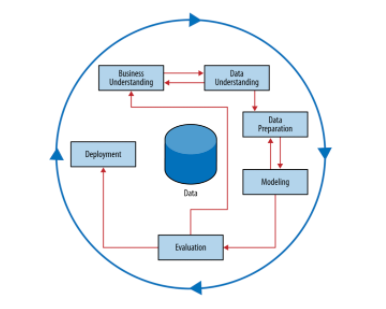
\includegraphics [scale= .95]  {CRISP.PNG}    %Include our ijmage with a height and location of img.
	\caption[Optional caption] {real, local caption for refrence}
	\label{fig:wordcloudBliz}

\end{figure}


The model serves to illustrate how the data was processed throughout the project in order to yield a final result/answer to the research questions. The model is iterative and serves to explore the Twitter data, so a better
understanding of the data can be reached. This process has been consciously iterated throughout the project.

"Business understanding" is in this context the overall problem formulation and research questions that we wish answered. For every iteration a deeper understanding of the data is achieved, which affects the understanding of the overall research framework.

Data Understanding is how we collect the data from raw material and build a solution, it is therefore essential to critique your data and see what strengths and weaknesses that the data has. It can also be relevant to estimate the cost of the data, especially in a business context. However, for the purposes of this specific research paper, the economical aspect of data collection such as Cost/benefit won't be explored. Due to the iterative nature of the CRISP framework, different solutions may change the direction of the analysis. The essential part to take away from this, is that we use data understanding in order to get a deeper understanding of our data and thus discover what the structure of the data is and how it can be used to "solve" what in this research paper is our business problem/research questions.

"Data preparation" is where we merge, cleanse and integrate multiple data sources. In this research paper, Alteryx has been used as shown in Table 1 later in the report.
"Modelling has used Tableau, which is a visual analytics tool. This makes it easier to explore and understand the patterns presented in the data. It has been a very closely fit process together with data understanding, in order to achieve the best results of "good" data (In this case, usable data that can answer our research questions)  and how to prepare it (So that frontend programs can be used in order to visualize  findings) \\

Modelling is what we end up with, it is here our overall "model" is made which captures patterns and regularities within the data. It is the stage where most data mining techniques are applied in order to create a model that is usable.

"Evaluation" Here we evaluate, whether the data model that has been built answers the overall research questions. After the model has been evaluated and validated, the model will go through "deployment", which in this sense will be the final conclusion to
the research questions.\\


\subsection{Process of Handling Data}

I have developed the following model, to illustrate how I have used Alteryx and Tableau in order to build a model. I have also attempted to illustrate how I used the CRISP model here, by determining if a given model is satisfactory. If not, I go back to the drawing board and reconsider what data I have and how I can prepare it in Alteryx, so that I can build a new model through the next iteration.



\begin{figure}[H] %We begin our figure and want it to stay H(ere)
	\centering %We want to center the figure
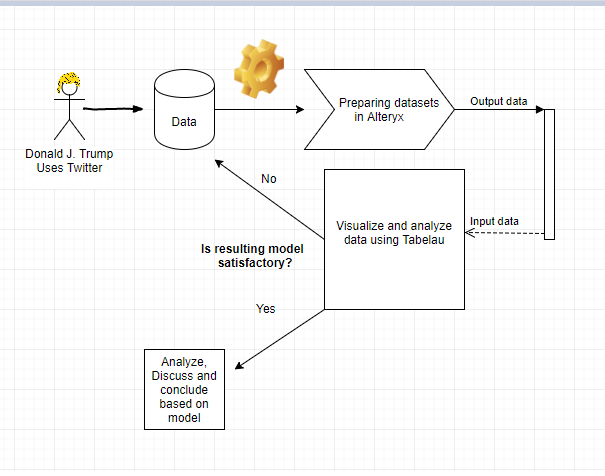
\includegraphics [scale= .85]  {SygModel.PNG}    %Include our ijmage with a height and location of img.
	\caption[Optional caption] {real, local caption for reference}
	\label{fig:wordcloudBliz}

\end{figure}


Throughout this project, I have attempted numerous models, most of which were discarded. Such as determining which fake news trump tweets most about, because I did not feel it answered the overall research question further.










%Table
%https://www.alteryx.com/analytics/data-mining-software

%Data Analytics tool that provide data mining solutions
% by helping with data cleansing and integration 
%of multiple sources.
%This tool helps with visual data representations in a 
%dynamic environment, where several datasets can be
%joined in order to create a comprehensive data solution.
 To summarize, Table 1 shows the purpose and use of each datamining tool used in this research paper: 


\begin{table}[H]
\centering
\caption{My caption}
\label{my-label}
\begin{tabular}{|l|l|l|l|l|}
\hline
\rowcolor[HTML]{656565} 
{\color[HTML]{000000} \textbf{Tool:}} & {\color[HTML]{000000} \textbf{Purpose:}} & \multicolumn{3}{l|}{\cellcolor[HTML]{656565}{\color[HTML]{000000} \textbf{Use:}}} \\ \hline
\rowcolor[HTML]{BBDAFF} 
\cellcolor[HTML]{BBDAFF}{\color[HTML]{000000} } & \cellcolor[HTML]{BBDAFF}{\color[HTML]{000000} } & \multicolumn{3}{l|}{\cellcolor[HTML]{BBDAFF}{\color[HTML]{000000} }} \\
\rowcolor[HTML]{BBDAFF} 
\cellcolor[HTML]{BBDAFF}{\color[HTML]{000000} } & \cellcolor[HTML]{BBDAFF}{\color[HTML]{000000} } & \multicolumn{3}{l|}{\cellcolor[HTML]{BBDAFF}{\color[HTML]{000000} }} \\
\rowcolor[HTML]{BBDAFF} 
\multirow{-3}{*}{\cellcolor[HTML]{BBDAFF}{\color[HTML]{000000} \textbf{Alteryx}}} & \multirow{-3}{*}{\cellcolor[HTML]{BBDAFF}{\color[HTML]{000000} \begin{tabular}[c]{@{}l@{}}Data Analytics tool that \\ provide data mining solutions\\  by helping with data \\ cleansing and integration \\ of multiple sources.\end{tabular}}} & \multicolumn{3}{l|}{\multirow{-3}{*}{\cellcolor[HTML]{BBDAFF}{\color[HTML]{000000} \begin{tabular}[c]{@{}l@{}}Lorem ipsumLorem ipsumLorem \\ ipsumLorem ipsum\\ Lorem ipsumLorem ipsumLorem ipsum\end{tabular}}}} \\ \hline
\rowcolor[HTML]{BBDAFF} 
\cellcolor[HTML]{BBDAFF}{\color[HTML]{000000} } & \cellcolor[HTML]{BBDAFF}{\color[HTML]{000000} } & \multicolumn{3}{l|}{\cellcolor[HTML]{BBDAFF}{\color[HTML]{000000} }} \\
\rowcolor[HTML]{BBDAFF} 
\cellcolor[HTML]{BBDAFF}{\color[HTML]{000000} } & \cellcolor[HTML]{BBDAFF}{\color[HTML]{000000} } & \multicolumn{3}{l|}{\cellcolor[HTML]{BBDAFF}{\color[HTML]{000000} }} \\
\rowcolor[HTML]{BBDAFF} 
\multirow{-3}{*}{\cellcolor[HTML]{BBDAFF}{\color[HTML]{000000} \textbf{Tableau}}} & \multirow{-3}{*}{\cellcolor[HTML]{BBDAFF}{\color[HTML]{000000} \begin{tabular}[c]{@{}l@{}}This tool helps with visual\\ data representation.\end{tabular}}} & \multicolumn{3}{l|}{\multirow{-3}{*}{\cellcolor[HTML]{BBDAFF}{\color[HTML]{000000} \begin{tabular}[c]{@{}l@{}}Lorem ipsumLorem ipsumLore\\ m iLorem ipsumpsumdasdLo\\ remLorem ipsum ipsum\end{tabular}}}} \\ \hline
\end{tabular}
\end{table}


\subsection{Data Acquisition and Dataset Description}
The first datasets consists of Twitter data on Trump's primary twitter channel.  This dataset will mainly be used to analyze Trump and his behavior on Twitter.

The second dataset was collected from Nasdaq and is used to collect information about the stock price of lockheed-martin, which is a company that Trump tweeted negatively about. 

The third dataset is collected through Sentione and will be used to analyze the sentiment towards Trump's campaign. Ranging from before his inauguration, until 02/11/2017. 


\section{Results}
In this section of the research paper, I will go through the results of my datamining and discuss it in relation to the research question, and thus explain which insights I came across during my datamining, in order to create a meaningful discussion regarding Donald J. Trump's behaviour and impact on the stock prices of companies. The result section will be built around the CRISP framework, in order to better illustrate the process of my datamining.

\subsection{Business understanding and Data Understanding}
The understanding of both the overall research questions / Problem statement and the data was a very iterative process and thus is hard to document in a research paper, therefore my understanding will mostly be reflected in the following sections, where my ideas and reflections will be discussed.  And hopefully create a reflection of how I arrived at the understanding of both my research questions and the data. \\

However, I would like to elaborate on the Data Understanding part, as this section includes evaluating the strengths and weaknesses of the data. In this research paper, Mostly data collected from Trump's twitter account has been collected, together with data on various stock prices on companies.  As mentioned by Provost and Fawcett, there is rarely an exact match between the overall problem and the data, thus this has to be kept in mind when reading the next sections. Other factors that may have contributed to the changes in stock prices from the analyzed companies is not within the scope of this research paper, nor is it in the datasets collected. Thus, this can be considered the weakness of the data. The strengths of the data however, is that there is enough variables within the dataset in order to make an analysis on Trump's behaviour, in addition, to be able to compare it to stock prices.

\subsection{Data Preparation}
In order to prepare the Datasets from Twitter and Sentione, I used a datamining tool called "Alteryx", which deals with the backend part of the data analysis. This tool was used to filter my data and join the relevant tables with each other, in order to make a comprehensive analysis. Data that was filtered out was things such as "Twitter ID" and "URL", as these were not needed for the direction I was going for. \\


One use of Alteryx was to do text-mining, which by nature is a very dirty and unstructured form of Big Data. While text-mining, it is important to keep in mind the context of the text (For example, what does Trump mean when he tweet "Crooked" a lot). Alteryx was used to find the frequency of the text, which shows how often a word showed up in the dataset.  \\

Figure X shows an algorithm created in Alteryx that allows the creation of word-clouds. This Algorithm filters the dataset, so it only presents the text values. Furthermore, the algorithm removes empty data entries as well as other noise from the data. (e.g. ! : ; ). Finally, the algorithm separates the sentences with new lines, so that every word can be counted by number of occurrence, this data can then be put into the Tableau software in order to create a WordCloud.



\begin{figure}[H] %We begin our figure and want it to stay H(ere)
	\centering %We want to center the figure
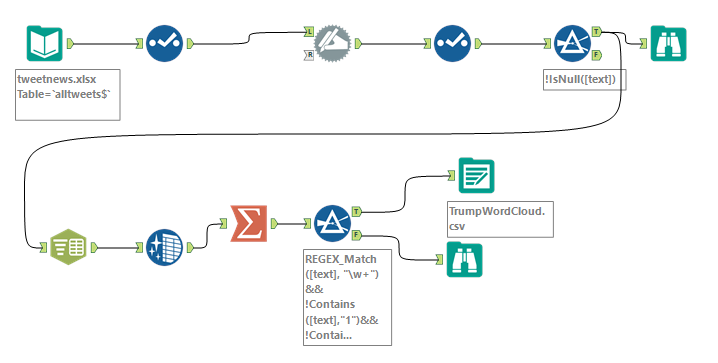
\includegraphics [scale= .65]  {TrumpWordCloudAlteryxFinal.PNG}    %Include our ijmage with a height and location of img.
	\caption[Optional caption] {real, local caption for refrence}
	\label{fig:wordcloudBliz}

\end{figure}

\subsection{Modelling, Evaluation and Deployment}
This section contains the models that I have produced with Tableau, which is the product i used to make my visual data analytics. In this section I will use the model to answer the research questions. \\

In order to answer the first research question, regarding Trump's behaviour before and after he announced his presidency, I used text-mining in order to build wordcloud, which shows which words he used frequently and thus can reveal something about his behaviour. The first model I want to show, is one that illustrates Trump's most used words before his announcement of candidacy.


\begin{figure}[H] %We begin our figure and want it to stay H(ere)
	\centering %We want to center the figure
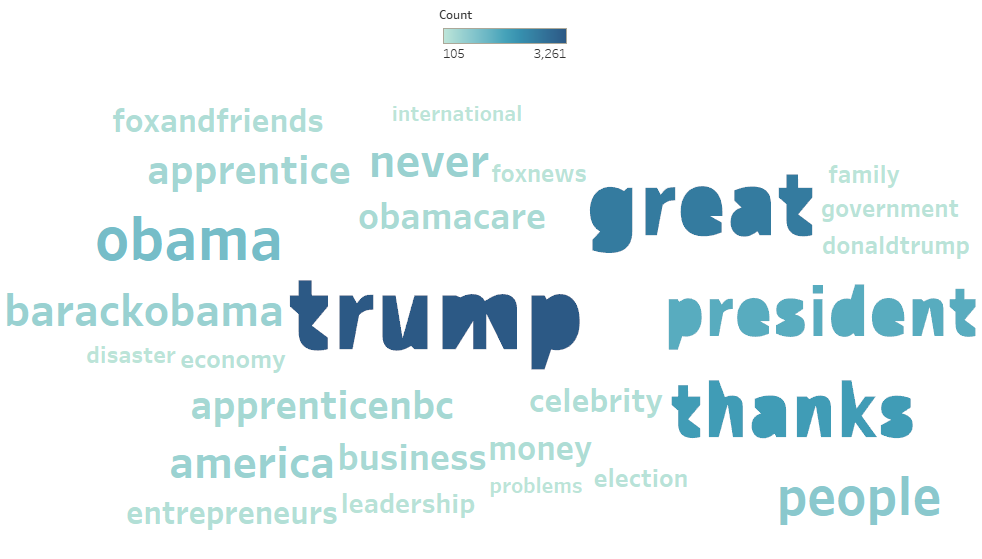
\includegraphics [scale= .45]  {TrumpBeforeAnnouncementWordFinal}    %Include our ijmage with a height and location of img.
	\caption[Optional caption] {real, local caption for refrence}
	\label{fig:wordcloudBliz}

\end{figure}

As Figure X shows, Trump was invested in the politics of USA before his announcement as president, having frequently used words such as "obamacare, president, government, barackobama". Furthermore, it can be seen that Trump's tweet weren't all about politics, but also about "business" and his TV-shows such as the apprentice (apprenticenbc). Therefore, it would be interesting to see a word-cloud of his behaviour after he announced his candidacy. 


\begin{figure}[H] %We begin our figure and want it to stay H(ere)
	\centering %We want to center the figure
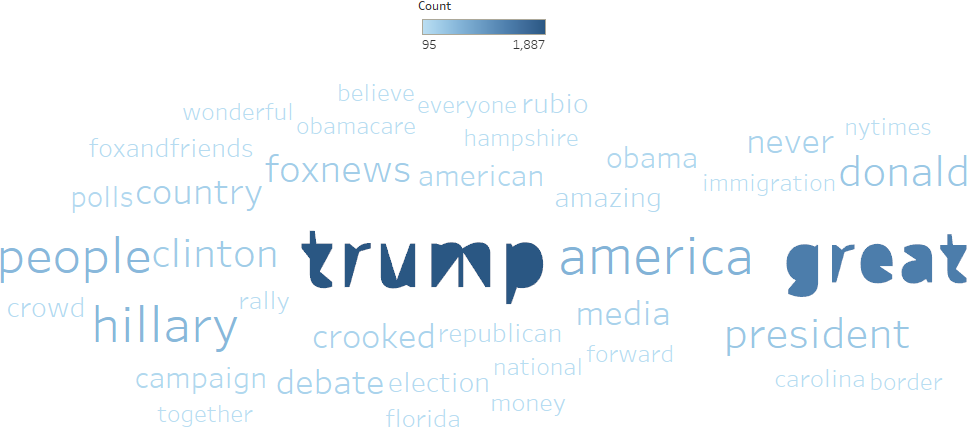
\includegraphics [scale= .45]  {TrumpAfterAnnouncement}    %Include our ijmage with a height and location of img.
	\caption[Optional caption] {real, local caption for refrence}
	\label{fig:wordcloudBliz}

\end{figure}

Here we see a similar, yet different story. Trump's tweets that were mostly unrelated to politics no longer showed up after filtering the word count, as they did in the previous model. Thus, we can see that Trump started focusing a lot more on politics and "fake news". Frequently using words such as "Hillary", "America", "media". We can also see, how Trump used twitter to further spread the nicknames of his political opponents, such as "crooked". \\

An interesting factor in this regard is to investigate the second research questions, so we can analyze how his behaviour on Twitter affected the "external environment", such as the stock prices of companies.  I created a model which illustrates how a negative tweet from Donald J. Trump, may affect the stock price of LockHeed Martin aircraft company.


\begin{figure}[H] %We begin our figure and want it to stay H(ere)
	\centering %We want to center the figure
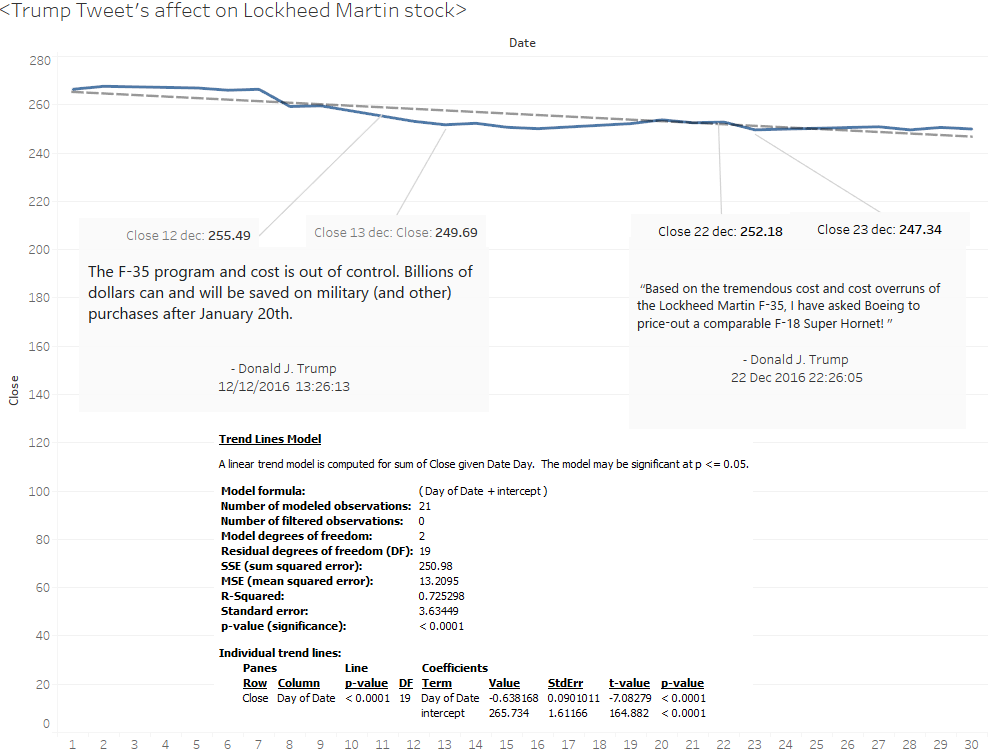
\includegraphics [scale= .45]  {lockfinal.png}    %Include our ijmage with a height and location of img.
	\caption[Optional caption] {real, local caption for refrence}
	\label{fig:wordcloudBliz}

\end{figure}

Figure X shows that the stock price before Trump posted a negative tweet, regarding his dissatisfaction with the F-35 program and how he would save money on military by cutting costs in the area that Lockheed Martin serviced the US.Army. As the graph shows, the closing price the day Trump made his tweet was 255.49 USD, but quickly fell to 249.69 USD the following day. Furthermore, later in the same month, Trump tweeted again that he would change supplier to Boeing, causing the stock price to fall from 252.18 to 247.34. \\

If we go further from this standpoint, we can make a linear regression of the month of December, where Trump made these tweets. The linear trend line shows a negative slope of -0.6 USD in close price every day, which shows that Trump's tweets did indeed have a negative impact on the stock prices of Lockheed Martin. Furthermore, it can be said that the model has an R-squared value of 0.725, which indicates that the goodness-of-fit for the datamodel is more or less decent. However, it should always be kept in mind as mention in the section "Theoretical Framework" that even a good R-squared value, may not always mean that you have a good model. \\

The above findings makes it interesting and relevant to expand our scope and look at the following month, to see if Trump's tweets' also affected the month of January 2017.

\begin{figure}[H] %We begin our figure and want it to stay H(ere)
	\centering %We want to center the figure
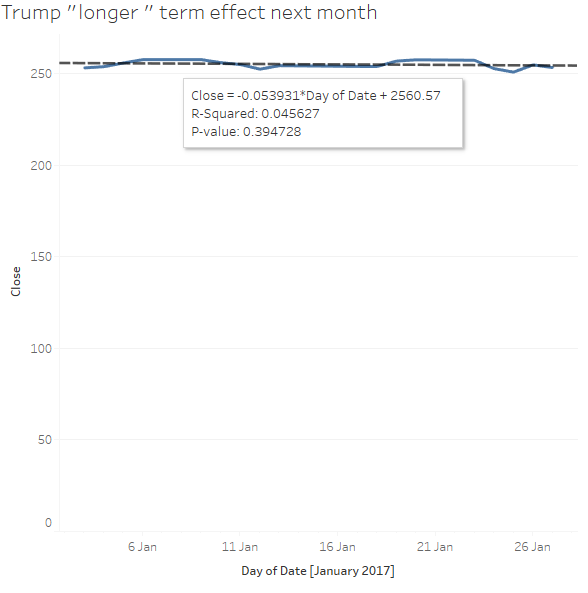
\includegraphics [scale= .6]  {TrumpJanuaryEffect.PNG}    %Include our ijmage with a height and location of img.
	\caption[Optional caption] {real, local caption for refrence}
	\label{fig:wordcloudBliz}

\end{figure}

It becomes clear that Trump's tweets' only have an initial effect on the market, as the stock quickly stabilized itself in the following month. However, one most keep in mind that this model has a very bad fit for our data, with an R-squared value of > 0.1, which means that it doesn't fit our observations in the data very well. 




\section{To be added later or thrown away}

Furthermore, by the use of text-mining and using an algorithm, that sorts comments into different classifications "positive", "negative", "neutral". It is possible to determine, whether the reaction of Trump's presidency was overall positive or negative. \\

The results show that Trump's initial support at the announcement of his presidency was overall positive, with very few negative comments.  The negative comments grew exponentially, as Trump got closed to winning his presidency, peaking around the time of his inauguration at xx/xx/xxxx


\section{Discussion}
I will now discuss the results and reflect upon them. As we saw in the models, Trump's tweet had a short-term negative effect on the Lockheed Martin stock in the month of December. This result was unsurprising, because he had won the election at that point and it was therefore likely that he could have a high impact on the F-35 program. In contrast though.

\subsection{Ethical discussion}

In order to discuss the findings in this research paper in relation to an important topic of Data Science, I will discuss what ethical issues that datamining and datascience have on society. According to Fawcett, there is a correlation between good business decisions and the use of data to base them on. As an example, a lot of information about Trump's behaviour was data-mined, revealing what topics he was interested in, what his impact is on his external environment etc. In Trump's case, he was mostly marketing his own "brand", but it is a concern, if such data was used on consumers without their consent and thus, raises questions about privacy. Companies will want to dig more and more into data about their consumers in order to reveal their behaviour and use it to increase the value in their business. This concern of privacy is a big issue, but is getting continuously regulated. As an example, a new personal data regulation in EU will help secure the privacy of consumers. http://ec.europa.eu/justice/data-protection/

\subsection{Learning reflection}
This research paper has helped me learn about the thought-process of a datascientist and how iterative the process is, as illustrated by the CRISP model. Unfortunately, I was unable to go as in-depth with the analysis as I wanted to, due to my limited knowledge of statistics and machine learning. In spite of all this, I do believe I arrived at some insights which allowed me to answer the research questions. In addition to this, the course and this research paper has taught me a lot about different analytics tools, which has given me a broad perspective of where I want to develop my skills in the future. Which for my case was in the realm of machine learning.


\section{Conclusion}
This research paper aimed to answer three different research questions: \\

\textit{What was trump's behaviour on social media, prior to his announcement of his presidency. And how did it change, during and after his political campaign.}\\

For this research question, text-mining was used in order to reveal the frequency and analyze the context, in which Trump's tweets contained. It was found, that Trump was invested in politics before and after he announced his candidacy. Although, Trump was more invested in his TV-shows, such as the Apprentice before his announcement. After his announcement, it was found that Trump had a much bigger focus on political statements, naming political opponents and negative nicknames for them. \\

\textit{How does Trump's behaviour affect the stock prices of companies ?} \\

This research question was answered using linear regression and data about a company in he aviation industry, called Lockheed Martin. It was here shown that Trump had a short-term effect on the stock price of the company, when he tweeted negatively about it. The findings showed that the following month, the stock-prices stabilized compared to the month of the tweets'.\\


\textit{What does using datascience to analyze Donald Trump's behaviour mean from an ethical standpoint?}\\
 
From an ethical standpoint, it was concluded that the possibility of using datamining and datascience to reveal the behavior and impact that an individual can have on social media, is a threat to the privacy in society. It was concluded that such areas must be regulated in order to protect the rights of privacy. Using regulations such as the personal data regulation in EU.  


\citep{blizzcon}

%End of report__________________________________

\cleardoublepage


\bibliographystyle{agsm}
\bibliography{mybib}

\cleardoublepage

\appendix
\section{\\Stests}

\end{document}






%\begin{figure}[H] %We begin our figure and want it to stay H(ere)
%	\centering %We want to center the figure


 %\raisebox{10mm}[0pt][0pt]{
%\fbox{ \makebox[\textwidth][c]{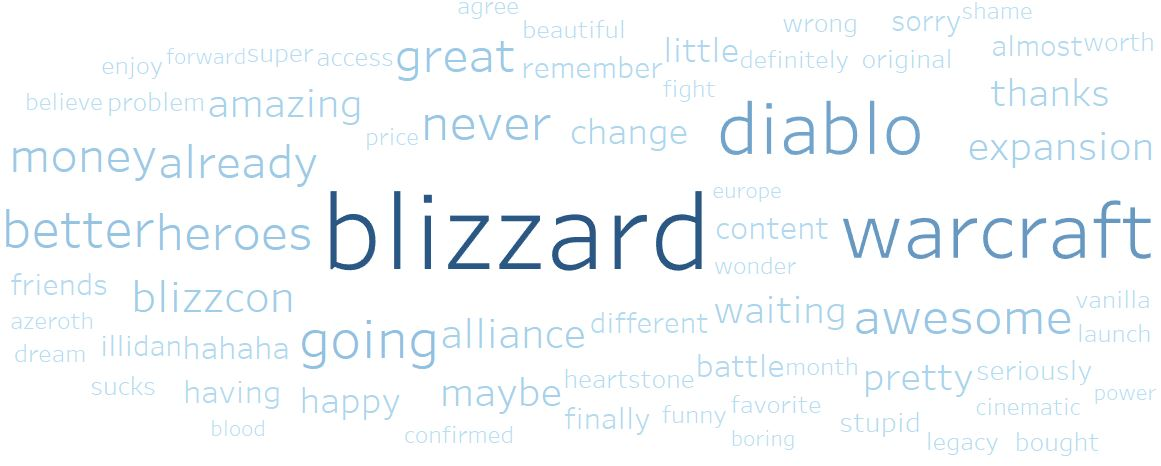
\includegraphics[scale=.55]{BlizzardWord2Cloud.PNG}}
% }}
%\vspace*{-40mm} %Close in the caption to the image

%\protect\caption[position=bottom]{Title of Figure\label{fig:F1}}


%\vspace{3cm}
%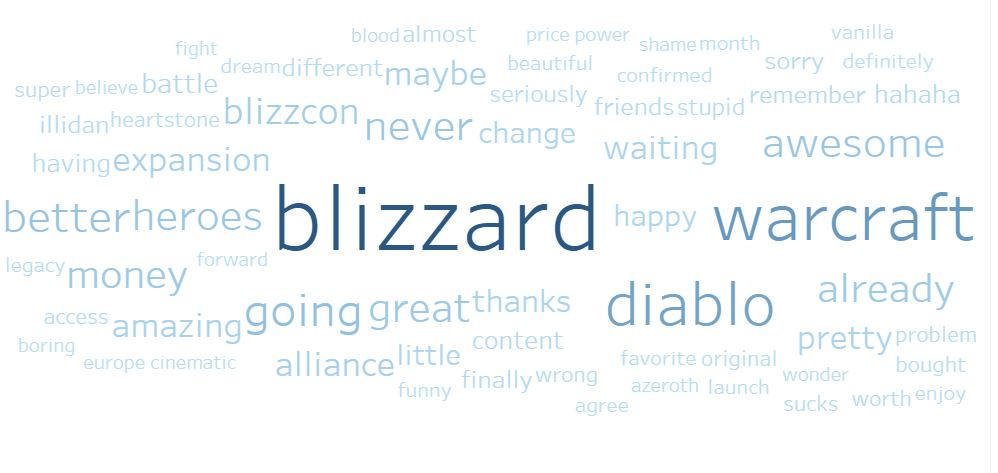
\includegraphics [width = 7in]  {BlizzardWordCloud.PNG}     %Include our ijmage with a height and location of img.
	
%	\label{fig:wordcloudBliz}

%\end{figure}



